\section{Data Distribution Service}

DDS is a messaging middleware standard \cite{dds-1.4-standard} for distributed applications. The standard is designed for mission- and business critical systems with real-time requirements. As such, DDS aims to function in a resource efficient and predictable manner, and is subject to minimal computational and transport overhead.\todo{benchmarks die das belegen?}

DDS is fundamentally based on the data-centric publish-subscribe (DCPS) paradigm. In the publish-subscribe-style communication, data flows between two kinds of entities: publishers and subscribers. Publishers offer data, while subscribers consume that data. A crucial characteristic of publish-subscribe is that data exchange between the peers is anonymous, \ie , publishers have no way of sending data to individual subscribers. Instead, both communicate by means of a shared, logical medium that takes data samples and forwards them to the appropriate receivers. In the context of DDS, this medium is called \emph{topic}. When subscribers receive a data sample they do not know where that sample originated. Similarly, publishers have no knowledge about where the sent data will end up at---or even if there are any receivers at all. Entities in this system find each other not by way of addressing, but rather on the basis of a shared understanding of what \emph{kind of data} they want to exchange. This approach is called \emph{data centricity}. Data centricity is in contrast to message centricity, in which data exchange is driven by \emph{messages}, or \emph{instructions}, which are directed at individual receivers. A prominent example of a message-centric technology is Remote Procedure Call (RPC). To illustrate the difference between the two paradigms consider \todo{direkte ansprache?} the example of a temperature sensor which propagates temperature data to multiple receivers. 

\todo[inline]{beispiel nicht so gut beschrieben}
In the message-centric paradigm, the sensor transmits data samples encapsulated in messages to the receivers. Messages are directed at each receiver individually, similar to a letter that is addressed to a certain postal address. For this, the sender needs to know the addresses of all interested receivers a-priori. The sender would have to maintain a list of receivers that it needs to update regularly. When a previously uninvolved entity decides to join the communication, it first needs to register to the sensor in order to make its address known. The sender would then have to add the address to its list of receivers. This causes overhead and makes the system inflexible and hard to scale.

In the DCPS approach, on the other hand, a subscriber that is interested in the sensor's data only knows that it wants to receive \emph{temperature data} while at the same time being entirely oblivious to the concept of \emph{temperature sensors}. 
Since publishers and subscribers have no references to one another, and know as little of each other as possible, a high level of loose coupling is achieved. This allows for a simple extension of the system, making it extraordinarily scalable.

Through the DCPS approach, DDS aims to provide a virtual \emph{global data space}. In this data space, data is universally accessible for all peers involved in the system. Data is not owned. 

Each component connected to the system views data as if it were available in a local storage, when in reality, it is distributed among many peers.


\paragraph{Programming Interface.}
The DDS standard specifies an API which is split into two separate parts. The main one, which is concerned with \emph{Data-Centric Publish-Subscribe} (DCPS), defines a low level API that enables basic DCPS-style message passing. The second part revolves around a \emph{Data Local Reconstruction Layer} (DLRL). DLRL sits on top of DCPS and is optional. The purpose of DLRL is to provide typed interfaces to messages. The delivered messages are conceived in a format suitable for direct processing in the application -- without the need to check the message's format. More precisely, DCPS performs a transformation of the unprocessed messages into language-specific data types. With the aid of DLRL, type-safety of communication is ensured and verification can be performed at compile-time, which helps to prevent bugs and reduces the application's error-proneness.


\paragraph{Decentralization.}
No single point of failure. No information brokers. no name servers.

\paragraph{Wire Protocol.}
The DDS standard does not dictate a wire protocol. DDS implementations may therefore utilize UDP, TCP and other protocols to exchange messages. This leaves room for ambiguity in the standard. As a result, DDS implementations are by default not interoperable. For this reason, a complementary wire protocol by the name of DDSI-RTPS\footnote{The "DDSI" in DDSI-RTPS is often omitted. The shortened form will henceforth be used.} (DDS Interoperability--Real-time Publish-Subscribe) was devised. Although RTPS is related to DDS, its specifics are outsourced in a separate standard. \cite{rtps-2.2-standard}

It uses the OMG \emph{Common Data Representation} (CDR) to encode data in a platform-neutral way. 

As a wire protocol, RTPS is deliberately tailored to DCPS-style communication among dispersed peers. In addition to the previously mentioned interoperability features, it provides multicast capabilities as means to enable simultaneous message delivery to several peers.

It also features multicast based service discovery.

RTPS is designed to work atop best-effort protocols, and in particular, UDP/IP. Because of the low overhead typical for such protocols, low latencies and high throughput can be achieved. However, the performance gain comes with tradeoffs, such as reduced reliability. The tradeoffs can be compensated by QoS settings. In a nutshell, RTPS is like an extension protocol to unreliable transports to make them more reliable, or rather, to allow for fine-grained control over the degree of the transport's reliability.



\paragraph{Bla}

data-centric instead of message-centric. The difference is that the former implies a shared data model. The middleware has an understanding of the data and its context and is responsible that all components have a common view of the data.
The advantage of data-centric messaging is that it allows a higher abstraction. Developers can focus on the data itself and on developing business logic instead of having to implement data sharing through exchange of messages.

DDS is a message bus. This is in contrast to a broker-based architecture. A broker enables flexible routing patterns featuring filtering, variable numbers of message queues etc. However, it can be considered a single point of failure.

peer discovery, transport methods, sampling rates, etc. are a matter of configuration


\begin{figure}[htpb]
  \centering
  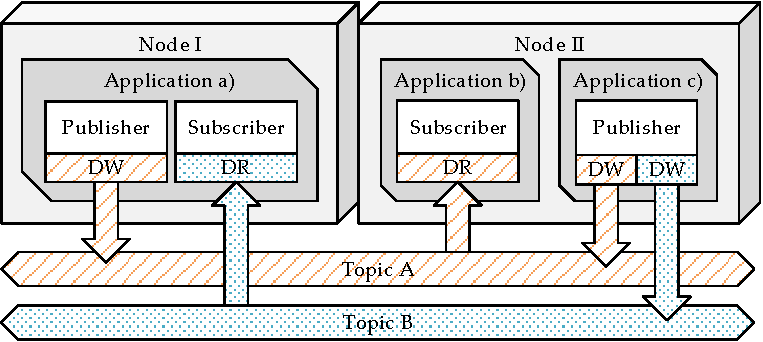
\includegraphics[width=0.8\textwidth]{figures/dds.pdf}
  \caption[An example of a distributed application connected via DDS]{An example of a distributed application connected via DDS}\label{fig:dds}
\end{figure}

\subsection{DDS Components}

The DDS specification defines a number of components for which it uses its own nomenclature. In the following, each component is described. \autoref{fig:dds} depicts an example highlighting how the components are related. In the example, there are two hardware nodes connected by an unspecified computer network. Each node can execute multiple applications simultaneously. The applications communicate with each other by means of DDS. 

\paragraph{Topics.}
\emph{Topics} form the basis on which peers communicate in the publish-subscribe paradigm. When a Publisher offers a certain kind of data, it does so by means of a Topic. When a data sample should be written, the Publisher pushes that data sample to a Topic appropriate for that sort of data. Conversely, when a Subscriber is interested in receiving data of a certain kind, then it subscribes to a Topic associated with that data. A Topic is defined by a unique identifier (name) and a data type. The data type represents the message format for messages sent over that Topic. For example, a suitable data type for a Topic concerned with temperature data would be a \texttt{struct} containing a single \texttt{float} value representing a temperature reading.

In \autoref{fig:dds}, two Topics are depicted (Topic A and Topic B), each with a number of associated Data Writers and Data Readers (see below). 

\paragraph{Publishers and Data Writers.}
\emph{Publishers} are entities that provide information in the publish-subscribe communication paradigm. Publishers are not bound to a single Topic. Instead, they contain one or more \emph{Data Writers}, each dedicated to a single Topic, who perform the actual message submission. Thus, Publishers may be seen as containers for a number of (unrelated) Data Writers. This concept is emphasized in \autoref{fig:dds} where a Publisher in Application c) controls two independent Data Writers that both write to different Topics.

\paragraph{Subscribers and Data Readers.}
\emph{Subscribers} are the exact compliment to Publishers in that they seek to receive data from Publishers. Analogous to Publishers, Subscribers are a way to group together sets of \emph{Data Readers}. Data Readers are entities whose purpose it is to receive messages from their respective Topic. Through its API, DDS allows Data Writers to receive data in three ways: either by waiting for messages (blocking the main thread), by pro-actively polling for new messages, or by specifying asynchronous callbacks which are invoked whenever a message arrives.

\paragraph{Domains and Domain Participants.}
\emph{Domains} are the DDS way of grouping together sets of coherent \emph{Domain Participants} and to separate those sets from each other. Speaking in terms of distributed systems, Domains are a mechanism to manage group memberships of nodes \cite{tanenbaum2017distributed}. 

Domain Participants are entities that belong to a particular Domain. Each Publisher, Subscriber and Topic is derived from one Domain Participant and is therefore dedicated to exactly that Domain. As a consequence, participants of different Domains are entirely separated from each other and there is no way for them to interface with each other. Depicted in \autoref{fig:dds} is only one Domain. However, there could just as well be other Domains. 


\subsection{Quality of Service}

\todo[inline]{get rid of term "service"}
One of DDS's salient features is its intrinsic QoS support realized by so-called \emph{QoS policies}. QoS policies specify service attributes for controlling each component's behavior and quality properties. They make specifying a service's attributes a matter of \emph{configuration}, rather than \emph{implementation}. For example, consider \todo{direkte ansprache?} a Data Writer which writes data to a Topic at a high rate. A Data Reader may be interested in that data but not at such a high rate, \eg\ because it runs on an embedded device powered by a battery and therefore needs to manage power consumption carefully. The Data Reader may now apply a \tbf , which instructs DDS to block all messages that exceed a specified frequency threshold. This way, the rate of incoming messages can be controlled via configuration. This is beneficial for the programmer as they do not need to accommodate for this at code level, but let the middleware take care of it.

QoS policies can be set for each Topic, Publisher, Subscriber, Data Writer and Data Reader individually. 
In \autoref{tab:qos}, an excerpt of the available QoS policies is given. For the exhaustive list of all available QoS policies refer to the official standard \cite{dds-1.4-standard}.

%
%
%
%
%
\begin{table}[H]
  \caption[An excerpt of DDS QoS policies]{An excerpt of QoS policies}\label{tab:qos}
  \centering
  \begin{tabular}{p{0.25\textwidth} p{0.2\textwidth}  p{0.45\textwidth}}
    \toprule
      \textbf{Name} & \textbf{Legal values} & \textbf{Description} \\
    \midrule
    	\reliability  & \texttt{RELIABLE}, \texttt{BEST\_EFFORT} & Indicates whether a Data Writer may drop samples or whether a Data Reader approves of Data Writers that drop samples.\\
    	\tbf  & An integer value denoting time & Specifies a Data Reader's desired data reception rate. Superfluous samples will be discarded.\\
    	\liveliness  & An integer value denoting time & Defines the rules to determine whether a particular entity is "alive", \eg\ by emitting heart beats. \\
    	\deadline  & An integer value denoting time & Establishes a contract between Data Writer and Data Reader to determine the acceptable data rate. \\
    	\ownership  & \texttt{SHARED}, \texttt{EXCLUSIVE} & Specifies whether multiple Data Writers may write to a given Topic simultaneously or just the one with the highest \ostrength\  value.\\
    	\ostrength  & An integer value denoting relative priority & Determines a Data Writer's priority in cases where its Topic's \ownership\ is set to \texttt{EXCLUSIVE}. \\
    	%\tpriority  & An integer value denoting relative priority &\\
    \bottomrule
  \end{tabular}
\end{table}
%
%
%
%
%

Another example of a QoS policy is the \deadline\ policy. It specifies the minimum message frequency of a service. If the deadline period of a hypothetical Data Writer is set to, e.g., 100 ms, then this Data Writer is obligated to send a message at least every 100 ms. If it fails to send messages at this rate, the Data Writer and all the respective Topic's readers will be notified about that circumstance and are free to act accordingly.

In addition to specifying quality attributes, QoS policies may also serve as service contracts. They specify non-functional requirements that services must fulfill to be able to communicate with each other. For example, a service provider's \reliability\ policy may have been set to the \texttt{BEST\_EFFORT} level, thereby allowing the service to drop samples. A service consumer, on the other hand, may require the service provider's policy to be set to \texttt{RELIABLE}, which prohibits the dropping of samples. Since the service provider only insufficiently fulfills the service consumer's QoS requirements, the services are considered incompatible with each other.

Despite their name, QoS policies do not only concern \emph{quality} attributes per se. They can also be used to specify the priority of messages, their lifespan, \ie , how long they are valid, or how many messages are kept in local memory.

\subsection{Implementations}
DDS, in itself, is only a standard. As such, DDS does not dictate, in detail, how to implement the concepts presented in the earlier sections. A number of DDS implementations from different vendors exist, all varying in terms of standard compliance, features beyond the standard, licensing, and other distinguishing factors. Compatibility between the respective implementations can be achieved by the use of the DDSI-RTPS wire protocol, which all major implementations support.

\paragraph{OpenDDS.}
Two types of discovery: centralized Information Repository, distributed RTPS discovery. The latter must be used if DDS implementation compatibility is priority

Only supports C++ and Java

\paragraph{OpenSplice.}


\paragraph{RTI.}
out of the implementations available to the broad public, it is by far the most mature and feature rich implementation.
Features encryption, compliance to several safety standards

%
%
%
%
%
%
%
%
%
%
%
%
%
%
%
%
%
%
%
%